\section{Using a Virtual Machine}

Just like a tree-walking interpreter, a virtual machine presents a method of implementing an interpreter for a programming language.
However, the way a virtual machine operates fundamentally differs from the one which the tree-walking interpreter uses.
For rush, we have implemented a virtual machine backend in order to compare it to the previously displayed tree-walking interpreter.

\subsection{Defining a Virtual Machine}

Often, one might encounter the term \emph{virtual machine} when talking about emulating an existing type of computer using a software system.
This emulation often includes simulating additional devices like the computer's display or its disk.
In this context however, a \emph{virtual machine} is a software entity which emulates how a computer interprets instructions.
Just like a real computer, a virtual machine executes low-level instructions directly.

Since a physical processor and a virtual machine share some fundamental traits,
the architecture of a virtual machine is often a slight deviation from the von Neumann architecture.
The von Neumann architecture was first introduced by John Neumann in the year 1945.
Von Neumann originally presented a design which allows implementing a computer using relatively few components.
A von Neumann computer usually contains components like an \emph{ALU}\footnote{Short for \enquote{arithmetic logic unit}}, multiple registers, a control unit, memory, and basic IO \cite[p.~172]{Ledin2020-yp}.
The ALU is designed in order to perform logical and mathematical operations as fast as possible.
However, in order to keep its implementation simple, it lacks the ability to fetch instructions from memory directly.
Therefore, a von Neumann processor contains a control unit which manages the \emph{fetch-decode-execute} cycle.
This cycle is a simplification of the steps a processor performs in order to execute instructions.

\begin{itemize}
	\item \textbf(Fetch): The processor's control unit loads the next instruction from the adequate memory location.
	      The value of the next instruction is then placed into the processor's internal instruction register.
	\item \textbf(Decode):
	      The processor's control unit examines the fetched instruction in order to determine if additional steps must be taken during instruction execution.
	      Such steps may involve accessing additional registers or memory locations.
	\item \textbf(Execute):
	      The control unit dispatches the instruction to a specialized component of the processor.
	      The target component is often dependent on the type of instruction since each processor component is optimized with one specific type of instruction in mind.
	      For instance, the control unit may invoke the ALU in order to perform a mathematical operation.
\end{itemize}

A computer's processor performs this fetch-decode-execute cycle repeatedly from the moment it is powered on until the point in time where it is powered down again.
For relatively simple processors, each cycle is executed in an isolated manner because instructions are executed in a sequential order.
This means that the execution of the instruction $i$ is delayed until execution of $i - 1$ has completed \cite[pp.~208-209]{Ledin2020-yp}.

For most virtual machines, executing the input instructions in sequential order is often the simplest solution.
Often, a virtual machine implements a method of instruction execution similar to the fetch-decode-execute cycle.
It is now apparent that a virtual machine is unable to traverse the AST directly and therefore relies on a sequence of instructions as its input.
Although the von Neumann architecture is relatively simple, one must not always adopt it when choosing how to implement a virtual machine.
Since virtual machines are purely abstract constructs, meaning that they are implemented using software, design constrains are usually kept to a minimum.
Therefore, designing an architecture of a virtual machine can sometimes be a demanding task.

\subsection{Register-Based and Stack-Based Machines}

One of the main decisions to be made when designing a VM is how it implements temporary storage.
Often, physical processors use \emph{registers} in order to make larger computations possible.
Registers are a limited set of very fast, low capacity storage units.
On modern architectures, like \emph{x86\_64}, each general-purpose register is able to hold as much as 64 bits of information.
However, there is always only a limited amount of registers available since they are physical components of the computers CPU.
Therefore, programs often only utilize registers for storing temporary values, such as intermediate results of a large computation.
The main alternative to using registers is a stack-based design.
A popular example for a stack-based virtual machine is \emph{WebAssembly}.
For compiler writers, register allocation is often a demanding task.
This problem is described in more detail in the later chapters. % TODO: refer to correct chapter
Since register allocation is not required in compilers generating code for stack-based machines, their implementation is often significantly easier compared to the one  of a compiler targeting a register-based machine.
Therefore, one might chose to implement a stack-based virtual machine in order to minimize complexity of both the compiler and the interpreter.
However, a stack-based design also introduces several issues on its own.
For instance, register-based machines might regularly outperform stack-based machines.
For instance, using the stack usually involves a lot of push or pop operations which could have otherwise been omitted.

\subsection{Comparing the VM to the Tree-Walking Interpreter}
A large benefit of virtual machines is that the source program runs significantly faster at runtime.
Therefore, implementing a programming language to run on a virtual machine is often a reasonable idea.
A reason for this speedup is that tree-traversal involves a lot of overhead which is omitted when interpreting instructions directly.

\TSListing[first line=5, caption={A Recursive rush Program}, label={lst:rush_vm_faster}, float=H]{listings/vm_faster.rush}
\noindent
\begin{figure}[h]
	\begin{minipage}{.7\textwidth}
		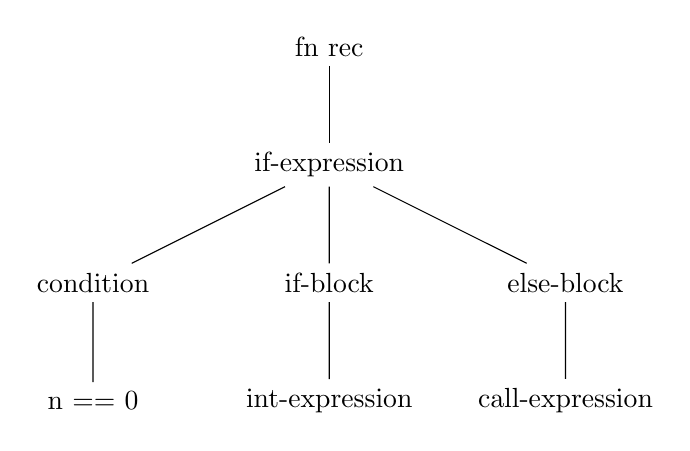
\begin{tikzpicture}[
				tlabel/.style={pos=0.4,right=-1pt,font=\footnotesize\color{red!70!black}},
			]
			\node{fn rec}
			child { node {if-expression}
					child { node {condition} child {node {n == 0}} }
					child [missing]
					child { node {if-block} child {node {int-expression}} }
					child [missing]
					child { node {else-block} child{node{call-expression}} }
				};
		\end{tikzpicture}
	\end{minipage}%
	\begin{minipage}{.3\textwidth}
		\TSListing[raw=true]{listings/vm_faster_instructions.txt}
	\end{minipage}
	\caption{Syntax Tree and VM instructions of a Recursive rush Program}
	\label{fig:tree_vs_vm}
\end{figure}

Figure \ref{fig:tree_vs_vm} displays a heavily simplified syntax tree and rush VM instructions representing the recursive program from above.
The root node of the syntax tree represents the \texttt{rec} function.
Since the function only contains a single expression, the if-expression node is the only child of the root node.
The if-expression contains a condition, an if-branch, and an else-branch.
Since the function should not call itself again if \texttt{n} is equal to 0, the if-block returns 0.
The else-block however calls the \texttt{rec} function recursively.
If the above program is executed, the tree-walking interpreter would have to traverse the entire tree of the \texttt{rec} function every time it is called.
Since \texttt{rec} is a recursive function, the tree-walking interpreter would have to traverse it $n$ times.
In this example, the syntax tree of the program is relatively simple.
However, the syntax tree of a more complex program will also contain more complexity.
Since loops and recursive functions execute the code in their bodies repeatedly, the tree traversal of the body presents an inefficiency.
Here, the inefficiency solely lies in the repeated tree-traversal, not in the repetition introduced by an iterative or recursive algorithm.
In order to improve efficiency, an algorithm could traverse the tree once, saving its semantic meaning in the process.
Then, the semantic meaning of the previously traversed tree could be interpreted repeatedly without the additional overhead.
The rush virtual machine operates exactly like this.
A compiler targeting the virtual machine's architecture first traverses the AST and outputs a sequence of instructions.
These instructions therefore represent the semantic meaning of the syntax tree.
Now, the virtual machine is able to interpret these instructions repeatedly with little additional overhead.
The instructions on the right side of figure \ref{fig:tree_vs_vm} represent the program in listing \ref{lst:rush_vm_faster}.
Everytime the \texttt{call} instruction in line 23 is executed, the VM only needs to jump to the instruction in line 10 in order to execute the \texttt{rec} function recursively.
Since repeated traversal of the syntax tree is omitted, rush programs will run significantly faster using the VM compared to the tree-walking interpreted.
Using the VM, executing the \texttt{rec} function using an input of $n = 1000$ took around 160 $\mu$s.
However, executing the identical code using the tree-walking interpreter took around 427 $\mu$s\footnote{Average from 10000 iterations. OS: Arch Linux, CPU: Ryzen 5 1500, RAM: 16 GB}.
Therefore, the rush VM executed the identical code roughly 2.6 times faster than the tree-walking interpreter.
However, the initial delay due to compilation is not considered in this benchmark.
As this example suggests, a virtual machine is often a rational way of implementing an interpreted programming language.

\subsection{The rush Virtual Machine}

The rush virtual machine is a stack-based interpreter implemented using the Rust programming language.
The machine's architecture is completely fictional and includes a \emph{stack} for storing short-term data, \emph{linear memory} for storing variables, and a \emph{call stack} for managing function calls.
Like most virtual machines, the rush VM implements a fetch-decode-execute cycle in order to interpret programs.

\TSListing[first line=13, last line=23, caption={Struct Definition of the \texttt{Vm}}, label={lst:vm_struct}, float=H]{deps/rush/crates/rush-interpreter-vm/src/vm.rs}

The instructions in figure \ref{fig:tree_vs_vm} can be interpreted by the rush VM.
Here, the output program is structured as functions which contain their instructions.
Because function names are replaced by indices, strings can be omitted in the output program which leads to a decrease in code size and an increase in runtime speed.
For better understanding, we have annotated the individual functions with a human-readable name.

The first block of instructions can be called the \emph{prelude} since its only task is to call the \texttt{main} function and declare global variables.
Global variables need to be initialized at the beginning of a program so that they can be accessed later in the program.
If global variables were present in the example, the prelude would contain the instructions used for initializing them.
If the prelude was omitted, the main function would instead contain these instructions since it is executed at program start.
However, recursion of the \texttt{main} function is legal in rush.
Therefore, each time the \texttt{main} function calls itself,
all global variables would be restored to their initial value since the initialization instructions are executed as well.
In order to prevent this bug, the rush VM uses a prelude function which is guaranteed to run only once.

Linear memory in the VM is represented as an infinitely growable list where each item saves the runtime value of a variable.
In the rush VM, each storage cell can be accessed using two addressing modes.
When using the \emph{absolute addressing} mode, the index of the target memory cell is specified.
For instance, if the value of variable \texttt{d} was to be retrieved, the VM would need to access the storage cell with the index 4.
However, the absolute position of a variable in memory can only be determined at runtime.
In a recursive function, each recursion adds more variables to the scope, thus allocating more memory.
Here, the exact number of recursions the function performs would have to be known at compile time.
Of course, this presents an impossible task, thus making writing a compiler targeting the VM impossible.
However, the rush VM also implements a \emph{relative addressing} mode which can be used without knowing the exact position of the target memory cell.
For instance, the value of variable \texttt{d} can be used by specifying that index 0 using relative addressing is to be retrieved.
In figure \ref{fig:rush_vm_linmem}, the memory pointer (shortened to \enquote{mp}) is set to 4.
Using the value of the memory pointer, the absolute address of any relative address can calculated at runtime.
Here, the absolute address $a$ is the sum of the relative index $i$ and the runtime memory pointer $m$.
Therefore, the absolute address of any relative address can be calculated at runtime like this: $a = i + m$.
By also implementing this relative addressing mode,
compilers targeting the rush VM can generate code without knowing the exact number of recursions a function performs.
In order to understand the difference between absolute and relative addressing modes, a practical example can be considered.
The code in listing \ref{lst:rush_pointer_simple} displays a rush program in which a pointer is created.
First, the integer variable \texttt{num} is created.
In line 3, a pointer variable called \texttt{to\_num} is created by \emph{referencing} the \texttt{num} variable.

\TSListing[caption={Minimal Pointer Example in rush}, label={lst:rush_pointer_simple}, float=H]{listings/simple_pointer.rush}

In the rush VM, absolute addressing is only used for global variables and pointers.
Since a pointer specifies the address of another variable, its runtime value will be the absolute address of its target variable.
In the VM, the absolute address of a variable is calculated as soon as it is referenced using the \texttt{\&} operator.
For this purpose, the \texttt{reltoaddr} instruction exists.
This instruction contains a parameter which specifies the relative address of the variable to be referenced.

\TSListing[raw=true, caption={VM Instructions for the minimal Pointer Example}, label={lst:rush_pointer_simple_vm_instructions}, float=H]{listings/vm_instructions_simple_pointer.txt}

The first instruction \texttt{setmp} increases the memory pointer by two.
This is because the \texttt{main} function contains two local variables whose space is to be allocated at the start of the function.
Therefore, one might encounter \texttt{mp} being incremented by 0 since the corresponding function contains no local variables.
The next instruction \texttt{push} pushes the value 42 onto the stack.
%: TODO: explain what svari does
Before a variable is referenced, its address is only saved as a relative addressing since the compiler is not aware of the absolute address at compile time.

\subsection{How the Virtual Machine Executes A rush Program}

In order to get a better understanding of how the rush VM works exactly, we will explain how it executes the program in listing \ref{lst:rush_vm_faster}.
For this, we should consider the instructions in figure \ref{fig:tree_vs_vm} again.
The first instruction of the prelude function is \texttt{setmp 0}.
This instruction adjusts the \emph{memory pointer} by the specified amount.
In this case however, the memory pointer remains unmodied since the argument of the instruction is 0.


\begin{figure}[h]
	\includegraphics[width=\textwidth]{./vm_linmem_draft.png}
	\caption{\textcolor{red}{DRAFT:} Linear Memory of the rush VM}
	\label{fig:rush_vm_linmem}
\end{figure}

Next, the \texttt{call 1} instruction calls the \texttt{main} function.
In order to understand how function calls work in this VM, we must consider the call stack of the rush VM.
Figure \ref{fig:compilation_steps} displays the state of the VMs call stack after the \texttt{call 1} instruction has been executed.
During execution of the call-instructions, the VM pushes a new stack frame onto its call stack.
Listing \ref{lst:call_frame_struct} shows how a call fram is implemented.
% TODO: explain fp / ip

\TSListing[first line=26, last line=31, caption={Struct Definition of a \texttt{CallFrame}}, label={lst:call_frame_struct}, float=H]{deps/rush/crates/rush-interpreter-vm/src/vm.rs}

\begin{figure}[h]
	\includegraphics[width=\textwidth]{./vm_call_stack_draft.png}
	\caption{\textcolor{red}{DRAFT:} Call Stack of the rush VM}
	\label{fig:rush_vm_call_stack}
\end{figure}
